% =============================================================================
%  FIVUCSAS  —  CSE4198 Engineering Project Poster  —  SHOWCASE variant
%  Marmara University, Department of Computer Engineering — Spring 2025-2026
%
%  Design goal: a product-showcase poster. Leads with a slogan, answers the
%  questions a visitor actually asks, and presents the value proposition,
%  the Top-10 feature set and the proof points — icon-driven, low text.
%
%  Visual assets:
%    assets/icons/*.pdf  — OpenMoji colour glyphs (CC BY-SA 4.0, hfg-gmuend/openmoji)
%                          + Tabler line icons (MIT) for fingerprint / qrcode / usb
%    assets/logos/*.pdf  — Simple Icons brand marks, brand-coloured
%    assets/*.{png,jpg}  — official Marmara University + Faculty crests
%
%  Compile:  pdflatex poster.tex && pdflatex poster.tex
% =============================================================================
\pdfminorversion=7  % allow inclusion of rsvg-convert PDF/1.7 assets
\documentclass[a0paper,portrait]{tikzposter}
\tikzposterlatexaffectionproofoff
\geometry{paperwidth=841mm,paperheight=1189mm}

% ---------- Packages ---------------------------------------------------------
\usepackage[utf8]{inputenc}
\usepackage[T1]{fontenc}
\usepackage{lmodern}
\usepackage{microtype}
\usepackage{graphicx}
\graphicspath{{./}{../../assets/}{../../assets/icons/}{../../assets/logos/}}
\usepackage{xcolor}
\usepackage{amsmath,amssymb}
\usepackage{fontawesome5}
\usepackage{qrcode}
\usepackage{tikz}
\usetikzlibrary{shapes.geometric,shapes.misc,arrows.meta,positioning,calc,fit,backgrounds}

% ---------- Marmara palette --------------------------------------------------
\definecolor{MarmaraNavy}{HTML}{0B2545}
\definecolor{MarmaraBlue}{HTML}{13315C}
\definecolor{MarmaraTeal}{HTML}{1E96A8}
\definecolor{MarmaraGold}{HTML}{F4B400}
\definecolor{MarmaraGray}{HTML}{E9ECEF}
\definecolor{MarmaraInk}{HTML}{1B1F23}
\definecolor{MarmaraSubtle}{HTML}{F6F8FB}
\definecolor{Spoof}{HTML}{C0392B}
\definecolor{Live}{HTML}{27AE60}

% ---------- Theme ------------------------------------------------------------
\definelayouttheme{MarmaraCSE}{
  \usecolorstyle[colorPalette=MarmaraStyle]{Default}
  \usebackgroundstyle{Default}
  \usetitlestyle{Filled}
  \useblockstyle{Default}
  \useinnerblockstyle{Default}
  \usenotestyle{Default}
}
\definecolorpalette{MarmaraStyle}{
  \definecolor{colorOne}{named}{MarmaraNavy}
  \definecolor{colorTwo}{named}{MarmaraBlue}
  \definecolor{colorThree}{named}{MarmaraTeal}
}
\usetheme{MarmaraCSE}
\colorlet{backgroundcolor}{MarmaraSubtle}
\colorlet{framecolor}{MarmaraNavy}
\colorlet{titlefgcolor}{white}
\colorlet{titlebgcolor}{MarmaraNavy}
\colorlet{blocktitlebgcolor}{MarmaraBlue}
\colorlet{blocktitlefgcolor}{white}
\colorlet{blockbodybgcolor}{white}
\colorlet{blockbodyfgcolor}{MarmaraInk}
\colorlet{innerblocktitlebgcolor}{MarmaraTeal}
\colorlet{innerblocktitlefgcolor}{white}

% ---------- Asset helpers ----------------------------------------------------
\newcommand{\ic}[2][3.2cm]{\raisebox{-0.15\height}{\includegraphics[height=#1,keepaspectratio]{#2}}}
\newcommand{\logo}[2][3cm]{\raisebox{-0.15\height}{\includegraphics[height=#1,keepaspectratio]{#2}}}
\newcommand{\unicrest}[1][3cm]{
\includegraphics[height=#1,keepaspectratio]{marmara-university.png}}
\newcommand{\faccrest}[1][3cm]{
\includegraphics[height=#1,keepaspectratio]{muhendislik-fakultesi.jpg}}

% ---------- Header info ------------------------------------------------------
\title{\parbox{0.97\linewidth}{\centering
  \begin{minipage}[c]{0.13\linewidth}\centering\unicrest[5.4cm]\end{minipage}\hfill
  \begin{minipage}[c]{0.70\linewidth}\centering
    {\fontsize{96}{100}\selectfont\bfseries FIVUCSAS}\\[0.18em]
    {\LARGE Face and Identity Verification Using Cloud-based SaaS}\\[0.30em]
    {\Large\textsl{A multi-tenant biometric identity platform\,---\,production-deployed}}
  \end{minipage}\hfill
  \begin{minipage}[c]{0.13\linewidth}\centering\faccrest[5.6cm]\end{minipage}
}}

\author{%
  \large \textbf{Ahmet Abdullah Gültekin} \quad
  \textbf{Ayşe Gülsüm Eren} \quad
  \textbf{Ayşenur Arıcı}\\[0.20em]
  \large \textbf{Advisor:} Assoc.\ Prof.\ Dr.\ Mustafa Ağaoğlu \, $\cdot$ \,
  CSE4197 / CSE4198 \, $\cdot$ \, Spring 2025--2026}
\institute{Marmara University \, $\cdot$ \, Faculty of Engineering \, $\cdot$ \, Department of Computer Engineering}

% =============================================================================
\begin{document}
\maketitle[width=\paperwidth, titletotopverticalspace=6mm]

% =================== SLOGAN HERO BAND ========================================
\block[bodyoffsety=-15mm, bodyinnersep=0mm]{}{%
\centering
\begin{tikzpicture}
  \node[fill=MarmaraNavy, rounded corners=16pt, minimum width=76cm, minimum height=12cm, inner sep=0pt] (s) {};
  \node[text=white, font=\fontsize{70}{76}\selectfont\bfseries] at ([yshift=22mm]s.center)
    {Register once.\ \ Verify everywhere.\ \ Every time.};
  \node[text=MarmaraGold, font=\fontsize{30}{34}\selectfont] at ([yshift=-26mm]s.center)
    {Ten authentication factors, one hosted login\,---\,protected by a liveness check a recorded video cannot fake.};
  \node at ([xshift=-330mm]s.center) {\ic[6.4cm]{user}};
  \node at ([xshift= 330mm]s.center) {\ic[6.4cm]{globe}};
\end{tikzpicture}}

% =================== WHAT FIVUCSAS SOLVES (full-width band) ==================
\block[titleoffsety=-10mm, bodyinnersep=6mm]{\faBullseye~~What FIVUCSAS solves}{%
\centering
\begin{tikzpicture}[every node/.style={align=center}]
  \foreach \px/\fx/\pain/\fix/\cx in {%
      key/puzzle/{Passwords leak,\\SIM-OTPs get swapped}/{10 composable factors\\in one MFA flow}/-28.5,
      video/shield/{Photos, clips \& deepfakes\\replay a face}/{Active randomised\\liveness challenge}/-9.5,
      scroll/check/{GDPR \& KVKK bolted on\\as an afterthought}/{Consent, export \&\\erasure built in}/9.5,
      gear2/link/{Re-integrating auth\\for every new app}/{One hosted OIDC\\for every platform}/28.5}{
    \node[font=\large\bfseries, text=Spoof, text width=15cm] at (\cx,3.0) {\pain};
    \node at (\cx-3.6,0.0) {\ic[3.0cm]{\px}};
    \node at (\cx-2.0,1.4) {\ic[1.3cm]{cross}};
    \draw[-Latex, line width=2.4pt, MarmaraNavy] (\cx-1.7,0) -- (\cx+1.7,0);
    \node at (\cx+3.6,0.0) {\ic[3.0cm]{\fx}};
    \node at (\cx+2.0,1.4) {\ic[1.3cm]{check}};
    \node[font=\large\bfseries, text=Live, text width=15cm] at (\cx,-2.9) {\fix};
  }
  \draw[MarmaraGray, line width=1.2pt] (-19,-3.6) -- (-19,3.8);
  \draw[MarmaraGray, line width=1.2pt] (  0,-3.6) -- (  0,3.8);
  \draw[MarmaraGray, line width=1.2pt] ( 19,-3.6) -- ( 19,3.8);
\end{tikzpicture}}

% ============================ COLUMNS ROW ====================================
\begin{columns}

% --------------------------- LEFT COLUMN -------------------------------------
\column{0.34}

\block{\faQuestionCircle~~Questions FIVUCSAS answers}{%
\begin{tikzpicture}[every node/.style={align=left}]
  \foreach \q/\a [count=\i] in {%
      {Is this a real person\\---\,or a replay?}/{Active liveness\,---\,0\,\% replay false-accept (n=120)},
      {Can one identity work\\across many apps?}/{Hosted OAuth2 / OIDC, tenant-scoped\,---\,redirect once},
      {Is my biometric\\data safe?}/{Facenet512 embeddings encrypted at rest\,---\,AES-128 Fernet},
      {Can I delete\\my data?}/{GDPR Art.\,17 erasure $+$ scheduled purge\,---\,KVKK aligned},
      {Do you verify real-world\\identity\,---\,not just login?}/{9-step pipeline: document $+$ NFC chip $+$ face $+$ liveness}}{
    \node[anchor=west] at (-11.0, {-(\i-1)*4.55}) {\ic[2.1cm]{check}};
    \node[anchor=west, font=\large\bfseries, text=MarmaraNavy] at (-8.6, {-(\i-1)*4.55+0.85}) {\q};
    \node[anchor=west, font=\normalsize, text=MarmaraInk, text width=18.8cm]
          at (-8.6, {-(\i-1)*4.55-1.15}) {\a};
    \ifnum\i<5 \draw[MarmaraGray, line width=1pt] (-11.0,{-(\i-1)*4.55-2.3}) -- (10.8,{-(\i-1)*4.55-2.3}); \fi
  }
\end{tikzpicture}}

\block{\faIndustry~~Built for nine industries}{%
\centering
\begin{tikzpicture}[every node/.style={align=center}]
  \foreach \i/\lbl/\x/\y in {%
      bank/Banking KYC/-9.0/1.9, hospital/Healthcare/-3.0/1.9,
      school/Education/3.0/1.9, govbuilding/Government/9.0/1.9,
      store/Retail age/-9.0/-2.4, briefcase/Corporate/-3.0/-2.4,
      airplane/Travel \& border/3.0/-2.4, creditcard/Fintech/9.0/-2.4}{
    \node at (\x,\y) {\ic[2.6cm]{\i}};
    \node[font=\normalsize\bfseries, text=MarmaraInk] at (\x,\y-1.9) {\lbl};
  }
\end{tikzpicture}\\[0.3em]
{\large Each industry ships as a ready \textbf{verification template}\,---\,steps, thresholds and regulators pre-wired.}
}

% --------------------------- MIDDLE COLUMN -----------------------------------
\column{0.32}

\block{\faStar~~Top 10 features}{%
\begin{tikzpicture}[every node/.style={align=left}]
  \foreach \icon/\title/\sub [count=\i] in {%
      key/{Ten composable auth factors}/{password $\cdot$ OTP $\cdot$ TOTP $\cdot$ QR $\cdot$ face $\cdot$ voice $\cdot$ NFC $\cdot$ WebAuthn},
      shield/{Active-liveness anti-spoofing}/{random facial-action challenge $+$ passive MiniFASNet},
      link/{Hosted OAuth2 / OIDC $+$ PKCE}/{redirective login, JWKS, discovery, RFC 8252 loopback},
      sliders/{Multi-tenant, tenant-controlled flows}/{each tenant composes its own MFA flow, no backend code},
      lock/{RBAC \& fine-grained permissions}/{roles, user-roles and permissions, row-level security},
      idcard/{9-step identity-verification pipeline}/{document scan $\to$ NFC chip $\to$ face match $\to$ liveness},
      briefcase/{7+ industry verification templates}/{Banking KYC, Healthcare, Gov e-KYC, Fintech\,\ldots},
      database/{Embedding encryption at rest}/{Fernet AES-128 wrap before pgvector write},
      scroll/{GDPR / KVKK compliance built in}/{consent, data export, right-to-erasure $+$ purge},
      mobile/{Every platform}/{web $\cdot$ Android $\cdot$ iOS $\cdot$ desktop $\cdot$ CLI}}{
    \node[circle, fill=MarmaraGold, text=MarmaraNavy, font=\Large\bfseries,
          minimum size=1.9cm, inner sep=0pt] at (-9.4, {-(\i-1)*3.05}) {\i};
    \node at (-6.7, {-(\i-1)*3.05}) {\ic[2.1cm]{\icon}};
    \node[anchor=west, font=\large\bfseries, text=MarmaraNavy]
          at (-5.2, {-(\i-1)*3.05+0.55}) {\title};
    \node[anchor=west, font=\small, text=MarmaraInk, text width=16cm]
          at (-5.2, {-(\i-1)*3.05-0.75}) {\sub};
    \ifnum\i<10 \draw[MarmaraGray, line width=0.8pt]
          (-10.4,{-(\i-1)*3.05-1.5}) -- (10.2,{-(\i-1)*3.05-1.5}); \fi
  }
\end{tikzpicture}}

% --------------------------- RIGHT COLUMN ------------------------------------
\column{0.34}

\block{\faChartBar~~By the numbers}{%
\centering
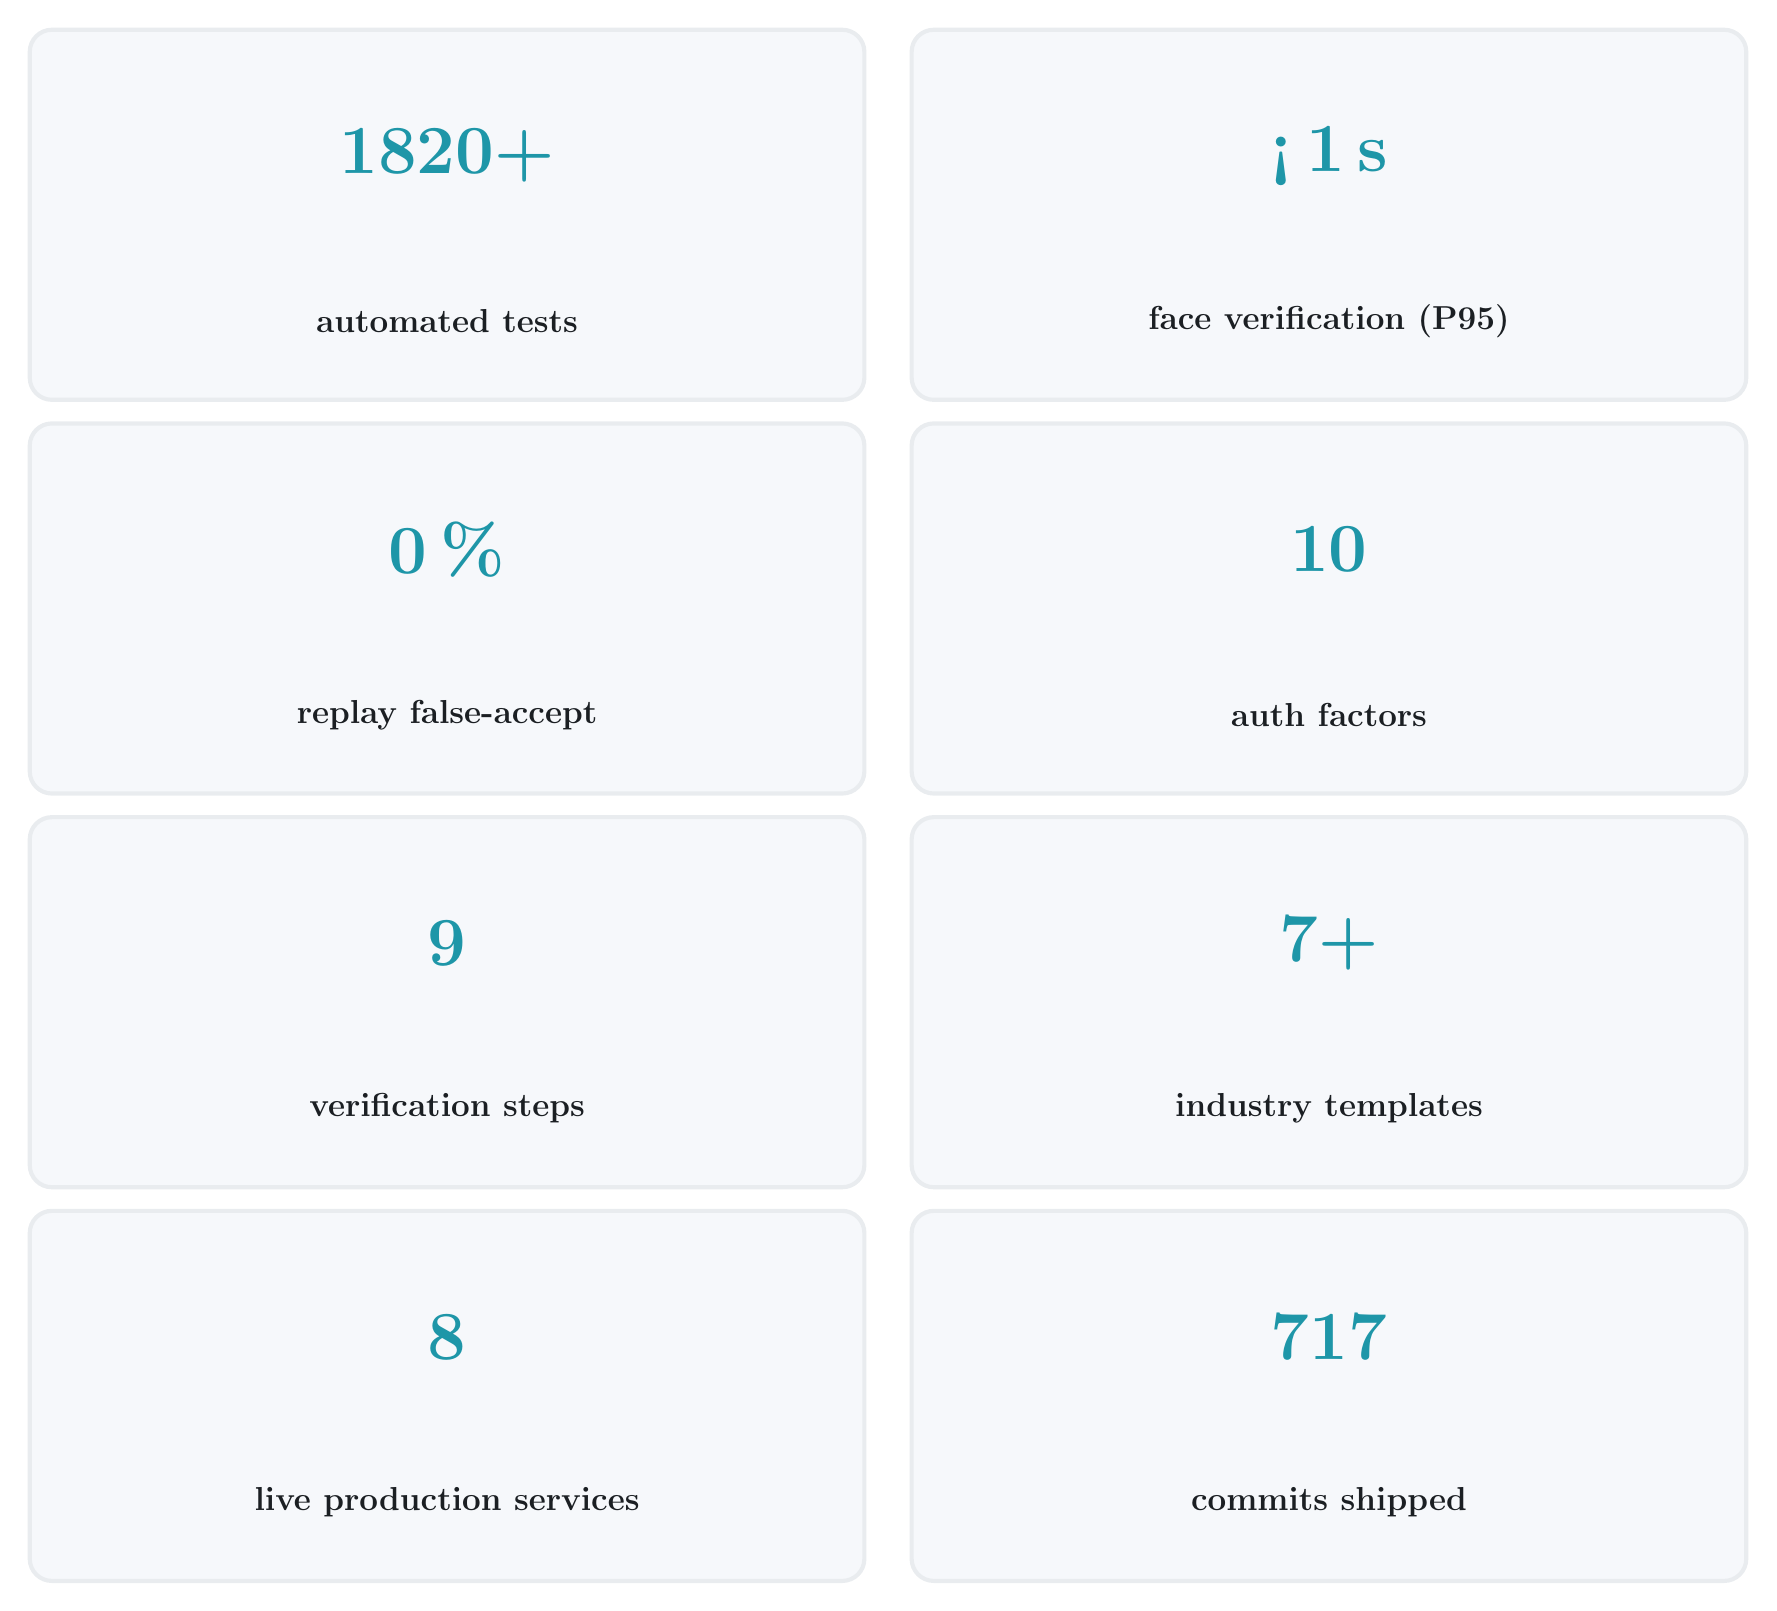
\begin{tikzpicture}[
  stat/.style={fill=MarmaraSubtle, draw=MarmaraGray, line width=1.5pt,
               rounded corners=8pt, minimum width=10.6cm, minimum height=4.7cm, inner sep=0pt},
  every node/.style={align=center}]
  \foreach \num/\lbl/\x/\y in {%
      {1820+}/automated tests/-5.6/7.05,
      {<\,1\,s}/face verification (P95)/5.6/7.05,
      {0\,\%}/replay false-accept/-5.6/2.05,
      {10}/auth factors/5.6/2.05,
      {9}/verification steps/-5.6/-2.95,
      {7+}/industry templates/5.6/-2.95,
      {8}/live production services/-5.6/-7.95,
      {717}/commits shipped/5.6/-7.95}{
    \node[stat] at (\x,\y) {};
    \node[font=\fontsize{50}{50}\selectfont\bfseries, text=MarmaraTeal] at (\x,\y+0.75) {\num};
    \node[font=\large\bfseries, text=MarmaraInk] at (\x,\y-1.35) {\lbl};
  }
\end{tikzpicture}}

\block{\faSitemap~~Architecture at a glance}{%
\centering
\begin{tikzpicture}[every node/.style={align=center, font=\normalsize}]
  \node[draw=MarmaraBlue, fill=white, rounded corners=6pt, line width=1.2pt,
        minimum width=10.4cm, minimum height=3.4cm] (api) at (-5.6,0)
        {\logo[2.0cm]{springboot}\\[2pt]\textbf{Identity Core}\\[-1pt]\small frozen OIDC contract};
  \node[draw=MarmaraTeal, fill=MarmaraTeal!8, rounded corners=6pt, line width=1.2pt,
        minimum width=10.4cm, minimum height=3.4cm] (bio) at (5.6,0)
        {\logo[2.0cm]{fastapi}\\[2pt]\textbf{Biometric ML}\\[-1pt]\small weekly-changing models};
  \draw[-Latex, line width=1.6pt, MarmaraNavy] (api) -- node[above,font=\small]{API-key} (bio);
  \node[font=\small, text=gray] at (0,-2.6) {split along the OIDC-contract vs.\ ML-iteration boundary};
\end{tikzpicture}\\[0.5em]
\logo[2.1cm]{react}\hfill\logo[2.1cm]{kotlin}\hfill\logo[2.1cm]{python}\hfill%
\logo[2.1cm]{postgresql}\hfill\logo[2.1cm]{redis}\hfill\logo[2.1cm]{docker}\hfill%
\logo[2.1cm]{traefikproxy}\\[0.3em]
{\normalsize Spring Boot 3.4 $\cdot$ Java 21 $\cdot$ FastAPI / Python 3.12 $\cdot$ React 18 $\cdot$ Kotlin MPP $\cdot$ Postgres 17 $+$ pgvector}
}

\block{\faRocket~~See it live}{%
\centering
\begin{minipage}[c]{0.38\linewidth}\centering
  \qrcode[height=6.0cm,version=4,level=H]{https://verify.fivucsas.com}\\[0.2em]
  {\small\faCamera~~scan to try it}
\end{minipage}\hfill
\begin{minipage}[c]{0.58\linewidth}
  {\large
  \faGlobe~~\texttt{fivucsas.com}\\[3pt]
  \faUserShield~~\texttt{verify.fivucsas.com}\\[3pt]
  \faThLarge~~\texttt{app.fivucsas.com}\\[3pt]
  \faCode~~\texttt{api.fivucsas.com}}
\end{minipage}
}

\end{columns}

% =============================== FOOTER STRIP ================================
\block[bodyinnersep=2mm, bodyverticalshift=0mm]{}{%
\colorbox{MarmaraNavy}{\parbox{0.985\linewidth}{\centering\color{MarmaraGold}%
\vspace{2mm}\bfseries\large
\faGithub~~\texttt{github.com/Rollingcat-Software/FIVUCSAS}
\quad$\cdot$\quad
\faGlobe~~\texttt{fivucsas.com}
\quad$\cdot$\quad
\faEnvelope~~\texttt{ahmetabdullahgultekin@gmail.com}
\quad$\cdot$\quad
Marmara University \, \textbf{2026}\vspace{2mm}}}}

\end{document}
